\documentclass[12pt,letterpaper]{article}
\usepackage{graphicx,textcomp}
\usepackage{natbib}
\usepackage{setspace}
\usepackage{fullpage}
\usepackage{color}
\usepackage[reqno]{amsmath}
\usepackage{amsthm}
\usepackage{fancyvrb}
\usepackage{amssymb,enumerate}
\usepackage[all]{xy}
\usepackage{endnotes}
\usepackage{lscape}
\newtheorem{com}{Comment}
\usepackage{float}
\usepackage{hyperref}
\newtheorem{lem} {Lemma}
\newtheorem{prop}{Proposition}
\newtheorem{thm}{Theorem}
\newtheorem{defn}{Definition}
\newtheorem{cor}{Corollary}
\newtheorem{obs}{Observation}
\usepackage[compact]{titlesec}
\usepackage{dcolumn}
\usepackage{tikz}
\usetikzlibrary{arrows}
\usepackage{multirow}
\usepackage{xcolor}
\newcolumntype{.}{D{.}{.}{-1}}
\newcolumntype{d}[1]{D{.}{.}{#1}}
\definecolor{light-gray}{gray}{0.65}
\usepackage{url}
\usepackage{listings}
\usepackage{color}

\definecolor{codegreen}{rgb}{0,0.6,0}
\definecolor{codegray}{rgb}{0.5,0.5,0.5}
\definecolor{codepurple}{rgb}{0.58,0,0.82}
\definecolor{backcolour}{rgb}{0.95,0.95,0.92}

\lstdefinestyle{mystyle}{
	backgroundcolor=\color{backcolour},   
	commentstyle=\color{codegreen},
	keywordstyle=\color{magenta},
	numberstyle=\tiny\color{codegray},
	stringstyle=\color{codepurple},
	basicstyle=\footnotesize,
	breakatwhitespace=false,         
	breaklines=true,                 
	captionpos=b,                    
	keepspaces=true,                 
	numbers=left,                    
	numbersep=5pt,                  
	showspaces=false,                
	showstringspaces=false,
	showtabs=false,                  
	tabsize=2
}
\lstset{style=mystyle}
\newcommand{\Sref}[1]{Section~\ref{#1}}
\newtheorem{hyp}{Hypothesis}

\title{Problem Set 3}
\date{Due: November 19, 2022}
\author{Applied Stats/Quant Methods 1}


\begin{document}
	\maketitle
	\section*{Instructions}
	\begin{itemize}
		\item Please show your work! You may lose points by simply writing in the answer. If the problem requires you to execute commands in \texttt{R}, please include the code you used to get your answers. Please also include the \texttt{.R} file that contains your code. If you are not sure if work needs to be shown for a particular problem, please ask.
	\item Your homework should be submitted electronically on GitHub.
	\item This problem set is due before 23:59 on Sunday November 19, 2023. No late assignments will be accepted.

	\end{itemize}

		\vspace{.25cm}
	
\noindent In this problem set, you will run several regressions and create an add variable plot (see the lecture slides) in \texttt{R} using the \texttt{incumbents\_subset.csv} dataset. Include all of your code.

	\vspace{.5cm}
\section*{Question 1}
\vspace{.25cm}
\noindent We are interested in knowing how the difference in campaign spending between incumbent and challenger affects the incumbent's vote share. \\


	\begin{enumerate}
		\item Run a regression where the outcome variable is \texttt{voteshare} and the explanatory variable is \texttt{difflog}. \\

	
\noindent 
\textbf{Answer}
		
		After we load our dataset into our working environment, we execute our regression
		model in which the incumbent's vote share is explained by the difference in campaign spending between incumbent and challenger. \\
		

		
		\textbf{Step 1:} We begin by outlining our hypotheses.
		
\textbf{Null hypothesis:}
		A difference in campaign spending between incumbents and challengers has no impact on incumbent vote share
		
\textbf{Alternative hypothesis: }
		A difference in incumbent campaign spending either increases (or decreases) their vote share 

	$$H_0: \beta = 0$$
	$$H_A: \beta \neq 0$$
%	\vspace{.05cm}


		\textbf{Step 2:} We run our regression in R
		
		\begin{verbatim}
		model <- lm(inc.sub$voteshare ~ inc.sub$difflog, data=inc.sub)		
		\end{verbatim}
		
		We then run a summary to check the coefficients
		
		\begin{verbatim}
		summary(model)
		
		Call:
		lm(formula = inc.sub$voteshare ~ inc.sub$difflog, data = inc.sub)
		
		Residuals:
		Min       1Q   Median       3Q      Max 
		-0.26832 -0.05345 -0.00377  0.04780  0.32749 
		
		Coefficients:
		Estimate Std. Error t value Pr(>|t|)    
		(Intercept)     0.579031   0.002251  257.19   <2e-16 ***
		inc.sub$difflog 0.041666   0.000968   43.04   <2e-16 ***
		---
		Signif. codes:  0 ‘***’ 0.001 ‘**’ 0.01 ‘*’ 0.05 ‘.’ 0.1 ‘ ’ 1
		
		Residual standard error: 0.07867 on 3191 degrees of freedom
		Multiple R-squared:  0.3673,	Adjusted R-squared:  0.3671 
		F-statistic:  1853 on 1 and 3191 DF,  p-value: < 2.2e-16
		
		\end{verbatim}
		
\textbf{Step 3: Conclusions:}
		
		We have evidence to support the view that a one unit increase in spending leads to a 0.04 unit increase in vote share for the incumbent party. The estimated coefficient is statistically differentiable from zero at the $\alpha=0.05$ level because the p-value $<$ 0.05 ($\approx $2e-16).
		

\newpage
		
		\item Make a scatterplot of the two variables and add the regression line. 	
		
		\lstinputlisting[language=R, firstline=84, lastline=98]{PS3_my_answers_NC.R}  
		
\begin{figure*}[h!]
			
	\centering
	\caption{\footnotesize Incumbent Vote Share as compared to Campaign Spending. Using ggplot.}
	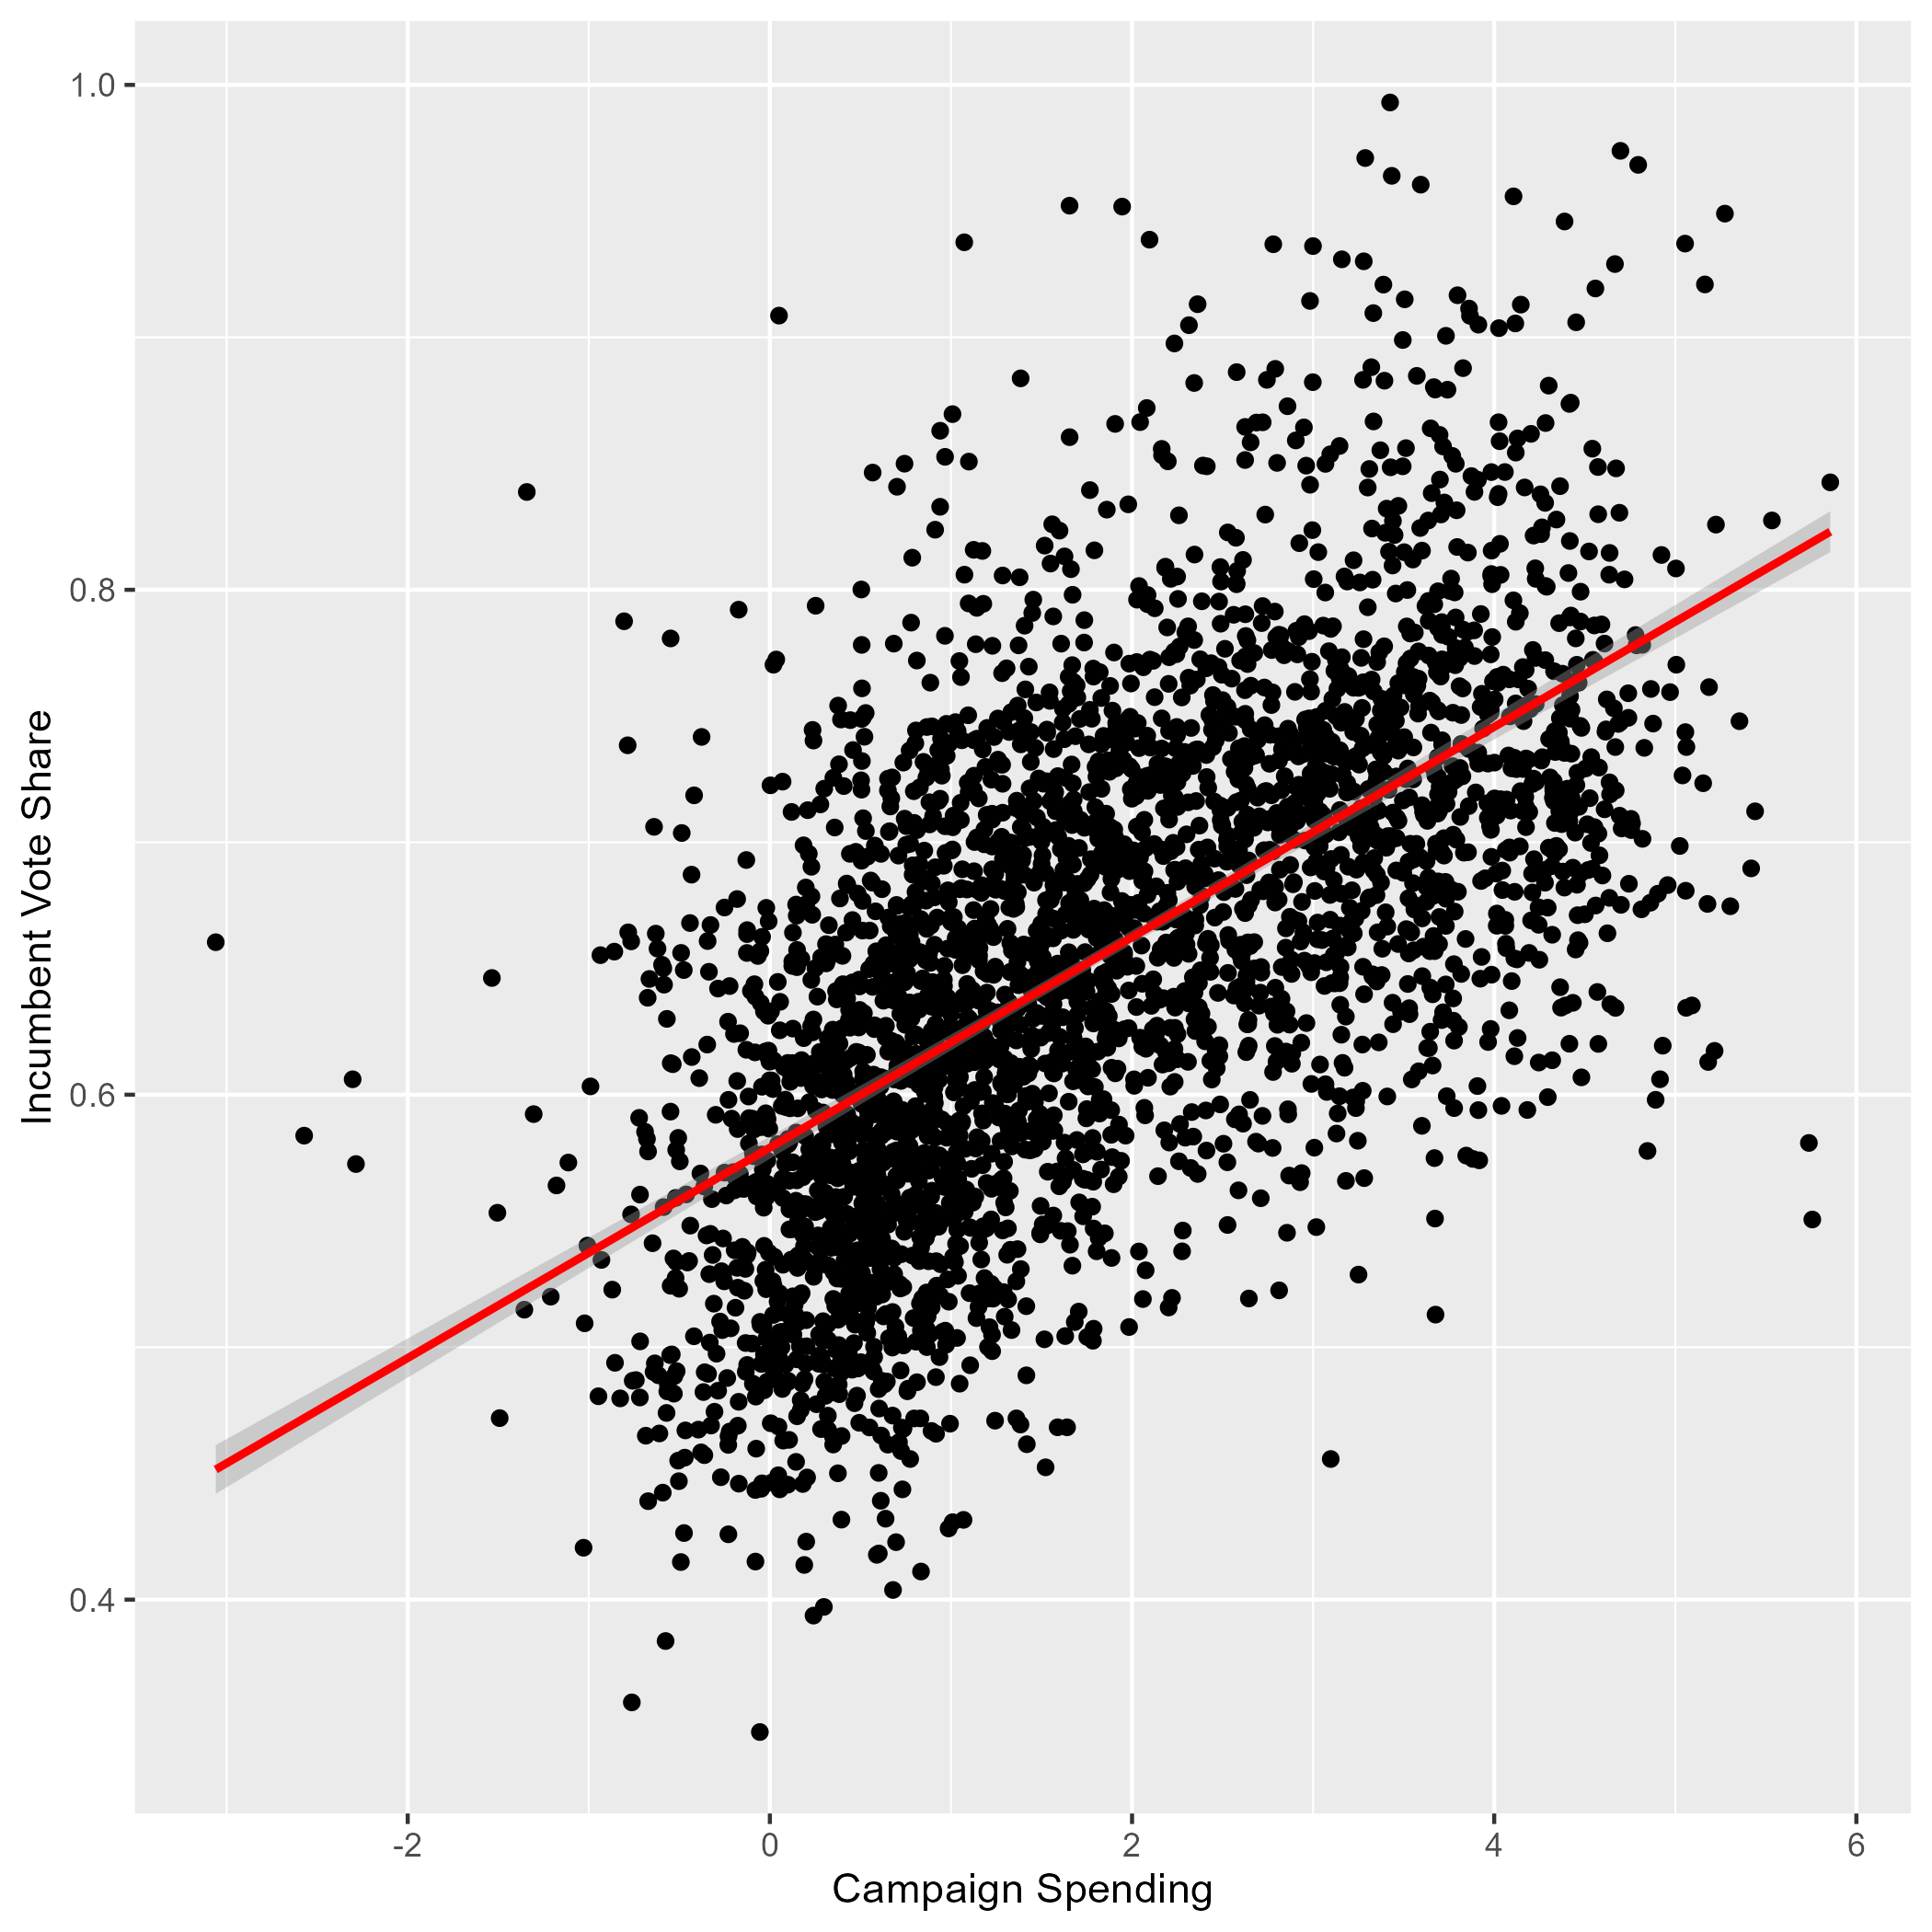
\includegraphics[width=0.79\textwidth]{vote_share_incumbent_scatter.png}
	
\end{figure*}

		
		
		
		\item Save the residuals of the model in a separate object.	
		
			\begin{verbatim}
vote_residuals <- model$residuals
vote_residuals
		\end{verbatim}
		
		\item Write the prediction equation.
		
			\end{enumerate}		
			
{\large 			$$\hat{Y}_i = \hat{\alpha} +  \hat{\beta}X_i $$}


{ 			$$\hat{Y}_i = 0.579031 +  0.041666 * \text{(Campaign Spending)} $$} \\

	
\noindent On average, with every additional dollar spent on the campaign, we can expect the vote share for the incumbent Party to increase by 0.041666 scale points. \\


	\newpage
	
	
\section*{Question 2}
\noindent We are interested in knowing how the difference between incumbent and challenger's spending and the vote share of the presidential candidate of the incumbent's party are related.	\vspace{.25cm}
	\begin{enumerate}
		\item Run a regression where the outcome variable is \texttt{presvote} and the explanatory variable is \texttt{difflog}. \\
		
		\noindent 
		\textbf{Answer}
		
		After we load our dataset into our working environment, we execute our regression
		model in which the presidential candidate of the incumbent's party vote share is explained by the difference in campaign spending between incumbent and challenger. \\
		
		
		
		\textbf{Step 1:} We begin by outlining our hypotheses. \\
		
		\textbf{Null hypothesis: }
		A difference in campaign spending between incumbents and challengers has no impact on the presidential candidate of the incumbent's party vote share \\
		
		\textbf{Alternative hypothesis: }
		A difference in campaign spending between incumbents and challengers either increases (or decreases) the vote share for the presidential candidate of the incumbent's party.
		
		$$H_0: \beta = 0$$
		$$H_A: \beta \neq 0$$
		%	\vspace{.05cm}
		
		\vspace{.25cm}
		
		
		\textbf{Step 2:} We run our regression in R
		
		\begin{verbatim}
		model_pres <- lm(inc.sub$presvote ~ inc.sub$difflog, data=inc.sub)

		\end{verbatim}
		
		We then run a summary to check the coefficients
		
		\begin{verbatim}
		summary(model_pres)

			
		Call:
		lm(formula = inc.sub$presvote ~ inc.sub$difflog, data = inc.sub)
		
		Residuals:
		Min       1Q   Median       3Q      Max 
		-0.32196 -0.07407 -0.00102  0.07151  0.42743 
		
		Coefficients:
		Estimate Std. Error t value Pr(>|t|)    
		(Intercept)     0.507583   0.003161  160.60   <2e-16 ***
		inc.sub$difflog 0.023837   0.001359   17.54   <2e-16 ***
		---
		Signif. codes:  0 ‘***’ 0.001 ‘**’ 0.01 ‘*’ 0.05 ‘.’ 0.1 ‘ ’ 1
		
		Residual standard error: 0.1104 on 3191 degrees of freedom
		Multiple R-squared:  0.08795,	Adjusted R-squared:  0.08767 
		F-statistic: 307.7 on 1 and 3191 DF,  p-value: < 2.2e-16
	
		\end{verbatim}
		
		\textbf{Step 3: Conclusions:}
		
		We have evidence to support the view that a one unit difference in spending leads to a 0.023837 unit change in vote share for the the presidential candidate of the incumbent's party. The estimated coefficient is statistically differentiable from zero at the $\alpha=0.05$ level because the p-value $<$ 0.05 ($\approx $2e-16). \\
		
		
		\item Make a scatterplot of the two variables and add the regression line. 	
		
		\lstinputlisting[language=R, firstline=162, lastline=176]{PS3_my_answers_NC.R}  
		
		\begin{figure*}[h!]
			\centering
			\caption{\footnotesize Presidential candidate of the incumbent's party vote share as compared to Campaign Spending. Using ggplot.}
			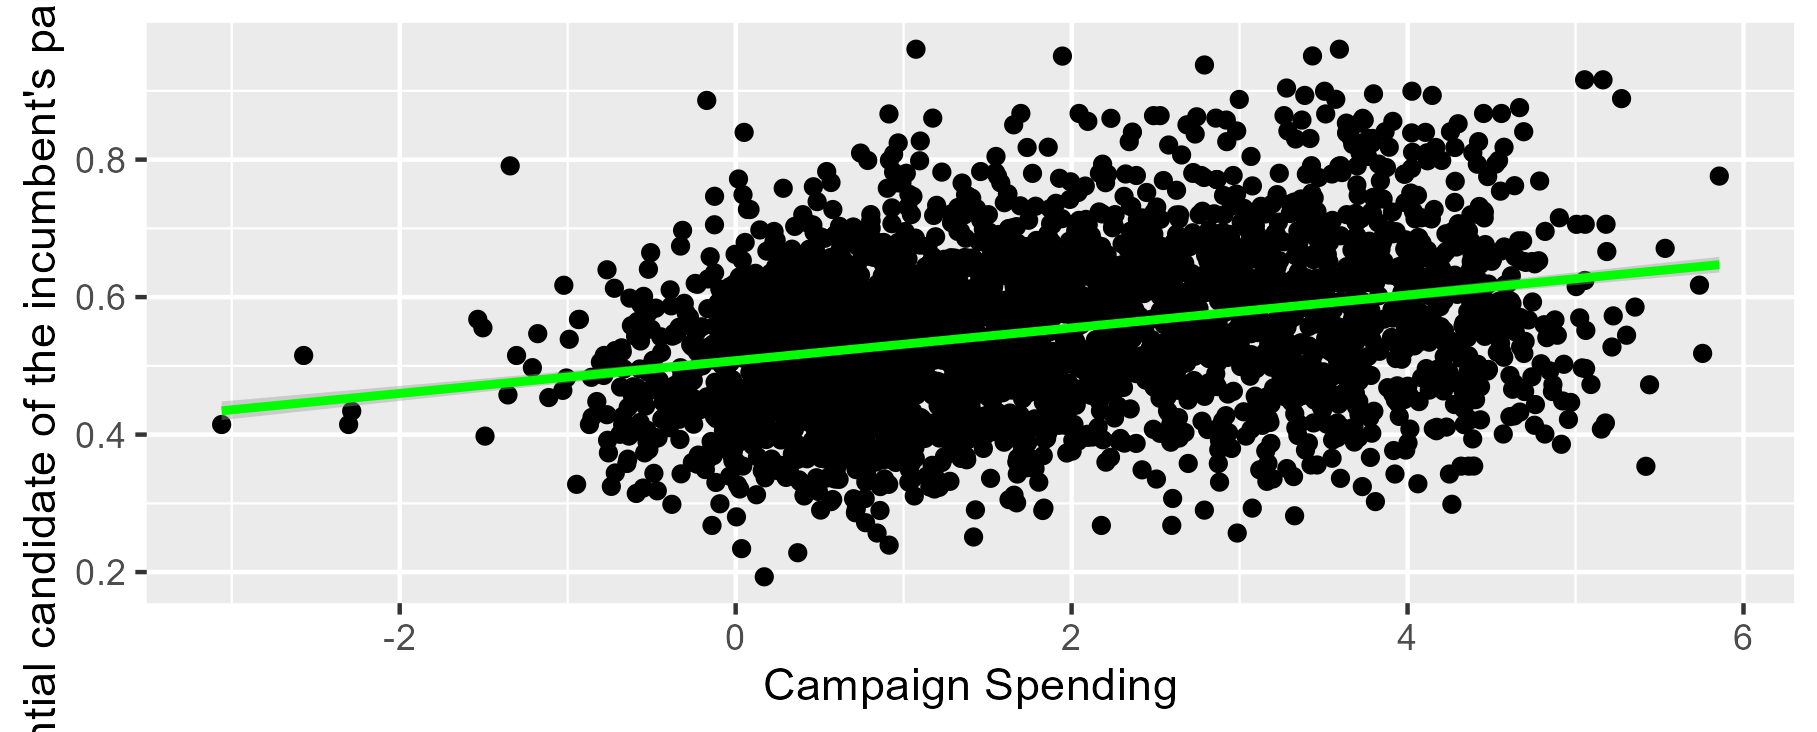
\includegraphics[width=0.99\textwidth]{vote_share_pres_scatter.png}
			
		\end{figure*} 
				
		\newpage
		
		\item Save the residuals of the model in a separate object.	
		
		\begin{verbatim}
			pres_residuals <- model_pres$residuals
			pres_residuals
		\end{verbatim}
		
		
		\item Write the prediction equation.
		
		\end{enumerate}		
		
		{\large 			$$\hat{Y}_i = \hat{\alpha} +  \hat{\beta}X_i $$}
		
		
		{ 			$$\hat{Y}_i =  0.507583 +  0.02383 * \text{(Campaign Spending)} $$} \\
		
	
	\noindent On average, with every additional dollar spent on the campaign, we can expect the vote share for the presidential candidate of the incumbent's party vote share to increase by 0.041666 scale points.
		

	
	\newpage	
\section*{Question 3}

\noindent We are interested in knowing how the vote share of the presidential candidate of the incumbent's party is associated with the incumbent's electoral success.
	\vspace{.25cm}
	\begin{enumerate}
		\item Run a regression where the outcome variable is \texttt{voteshare} and the explanatory variable is \texttt{presvote}. \\
	
\noindent 

	\textbf{Answer}
	
	After we load our dataset into our working environment, we execute our regression
	model in which we check for association between the vote share of the presidential candidate of the incumbent's party and the incumbent's electoral success. \\
	\\
	
	\textbf{Step 1:} We begin by outlining our hypotheses. \\
	\\
	
	\textbf{Null hypothesis: }
	There is no association between the vote share of the presidential candidate of the incumbent’s party and the incumbent’s electoral success \\
	\\
	
	\textbf{Alternative hypothesis: }
	There is an association between the vote share of the presidential candidate of the incumbent’s party and the incumbent’s electoral success
	
	$$H_0: \beta = 0$$
	$$H_A: \beta \neq 0$$
	%	\vspace{.05cm}
	
	\vspace{.25cm}
	
	
	\textbf{Step 2:} We run our regression in R

	
	\begin{verbatim}
		model <- lm(inc.sub$voteshare ~ inc.sub$presvote, data=inc.sub)		
	\end{verbatim}
	
	We then run a summary to check the coefficients
	
	\begin{verbatim}
		summary(model_pres)
		
		Call:
		lm(formula = inc.sub$voteshare ~ inc.sub$presvote, data = inc.sub)
		
		Residuals:
		Min       1Q   Median       3Q      Max 
		-0.27330 -0.05888  0.00394  0.06148  0.41365 
		
		Coefficients:
		Estimate Std. Error t value Pr(>|t|)    
		(Intercept)      0.441330   0.007599   58.08   <2e-16 ***
		inc.sub$presvote 0.388018   0.013493   28.76   <2e-16 ***
		---
		Signif. codes:  0 ‘***’ 0.001 ‘**’ 0.01 ‘*’ 0.05 ‘.’ 0.1 ‘ ’ 1
		
		Residual standard error: 0.08815 on 3191 degrees of freedom
		Multiple R-squared:  0.2058,	Adjusted R-squared:  0.2056 
		F-statistic:   827 on 1 and 3191 DF,  p-value: < 2.2e-16
		
	\end{verbatim}
	
	\textbf{Step 3: Conclusions:}
	
	We have evidence to support the view that a one unit increase in the incumbent party's electoral success leads to a 0.388 increase in vote share for the President's Party. The estimated coefficient is statistically differentiable from zero at the $\alpha=0.05$ level because the p-value $<$ 0.05 ($\approx $2e-16). \\
	
	
	\item Make a scatterplot of the two variables and add the regression line. 	
	
	\lstinputlisting[language=R, firstline=225, lastline=236]{PS3_my_answers_NC.R}  
	
	\begin{figure*}[h!]
		\centering
		\caption{\footnotesize President Party's Vote Share as compared to Incumbent's electoral success. Using ggplot.}
		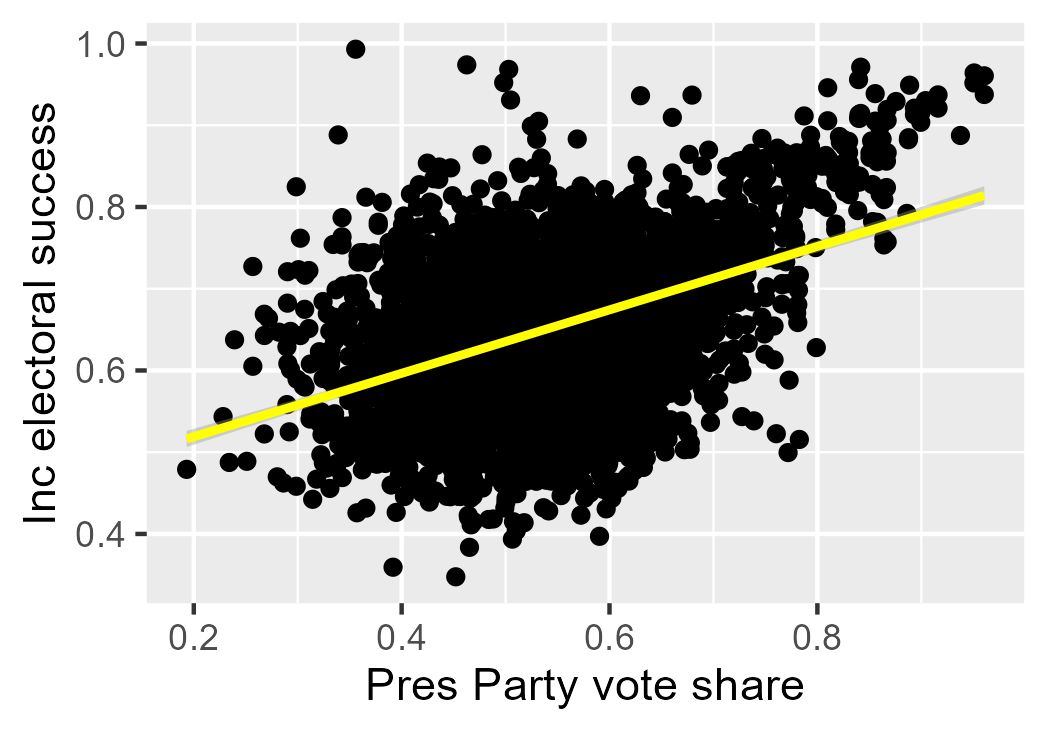
\includegraphics[width=0.99\textwidth]{vote_share2_scatter.png}
		
	\end{figure*} 
	
	\newpage
	
	\item Save the residuals of the model in a separate object.	
	
	\begin{verbatim}
		new_vote_residuals <- model_vote$residuals
		
	\end{verbatim}
	
	
	\item Write the prediction equation.
	
\end{enumerate}		

{\large 			$$\hat{Y}_i = \hat{\alpha} +  \hat{\beta}X_i $$}


{ 			$$\hat{Y}_i =  0.441330 +  0.388 * \text{(incumbent electoral success)} $$} \\


\noindent On average, with every one unit of electoral success for incumbent party, we can expect the vote share for the President's Party to increase by 0.388 scale points.\\

With regard to association, the slope is positive, indicating a positive association. The slope does not however tell us the strength of the association. \\

If we look at the $R^2$ value, it is 0.2058, indicating a weak positive relationship between the two variables.




\newpage	
\section*{Question 4}
\noindent The residuals from part (a) tell us how much of the variation in \texttt{voteshare} is $not$ explained by the difference in spending between incumbent and challenger. The residuals in part (b) tell us how much of the variation in \texttt{presvote} is $not$ explained by the difference in spending between incumbent and challenger in the district.
	\begin{enumerate}
		\item Run a regression where the outcome variable is the residuals from Question 1 and the explanatory variable is the residuals from Question 2.	\\
		
\textbf{		Null hypothesis: }
		There is no association between the residuals
		
\textbf{		Alternative hypothesis: }
		There is an association between the residuals \\

	$$H_0: \beta = 0$$
$$H_A: \beta \neq 0$$
%	\vspace{.05cm}

\vspace{.25cm}


Step 1: Run the regression ...

			\begin{verbatim}
model_residuals <- lm(pres_residuals ~ vote_residuals, data=inc.sub)

summary(model_residuals)


Call:
lm(formula = pres_residuals ~ vote_residuals, data = inc.sub)

Residuals:
Min       1Q   Median       3Q      Max 
-0.32618 -0.07532 -0.00485  0.06698  0.45288 

Coefficients:
Estimate Std. Error t value Pr(>|t|)    
(Intercept)    -2.874e-18  1.928e-03    0.00        1    
vote_residuals -2.059e-01  2.188e-02   -9.41   <2e-16 ***
---
Signif. codes:  0 ‘***’ 0.001 ‘**’ 0.01 ‘*’ 0.05 ‘.’ 0.1 ‘ ’ 1

Residual standard error: 0.1089 on 3191 degrees of freedom
Multiple R-squared:  0.027,	Adjusted R-squared:  0.02669 
F-statistic: 88.54 on 1 and 3191 DF,  p-value: < 2.2e-16

		\end{verbatim}
		
The slope is equal to -2.059e-01. So we do not have enough evidence to reject the null hypothesis in this instance. Note that the estimated coefficient is statistically differentiable from zero at the $\alpha=0.05$ level because the p-value  $<$ 0.05 ($\approx $2e-16).
	
		\item Make a scatterplot of the two residuals and add the regression line.
		
	\lstinputlisting[language=R, firstline=280, lastline=294]{PS3_my_answers_NC.R}  
			
	\begin{figure*}[h!]
	\centering
	\caption{\footnotesize Comparison of Residuals Using ggplot.}
	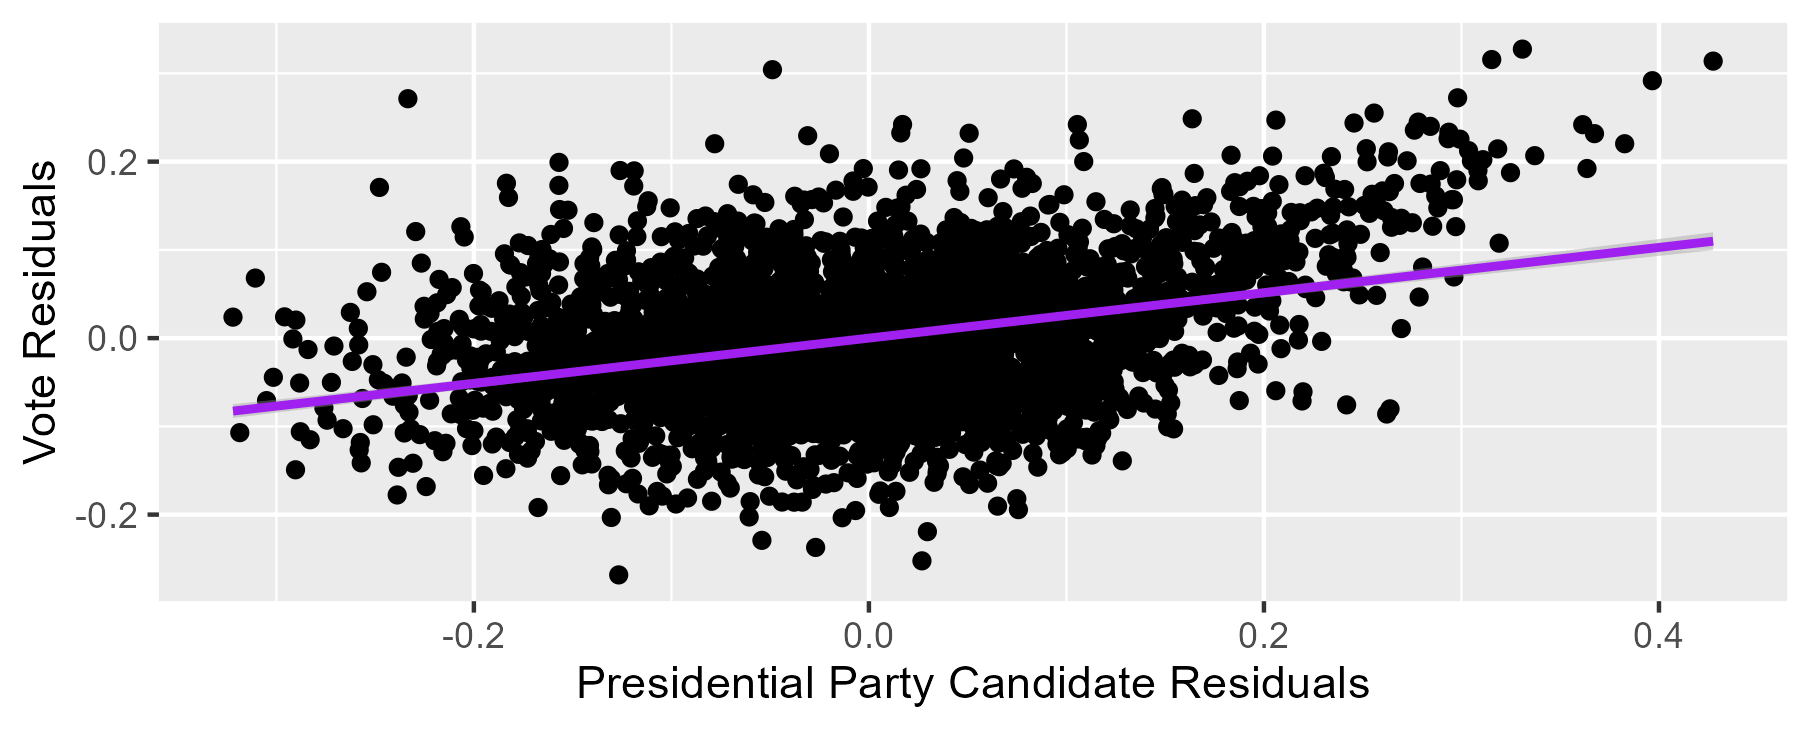
\includegraphics[width=0.99\textwidth]{residuals_scatter.png}
	
\end{figure*} 
		 
		\item Write the prediction equation.
		
		{\large 			$$\hat{Y}_i = \hat{\alpha} +  \hat{\beta}X_i $$}
		
		
		{ 			$$\hat{Y}_i =  -2.874e-18 +  -2.059e-01 * \text{(Residuals from part b)} $$} \\
		
	\end{enumerate}
	
	\newpage	

\section*{Question 5}
\noindent What if the incumbent's vote share is affected by both the president's popularity and the difference in spending between incumbent and challenger? 
	\begin{enumerate}
		\item Run a regression where the outcome variable is the incumbent's \texttt{voteshare} and the explanatory variables are \texttt{difflog} and \texttt{presvote}.	\vspace{5cm}
		\item Write the prediction equation.	\vspace{5cm}
		\item What is it in this output that is identical to the output in Question 4? Why do you think this is the case?
	\end{enumerate}

\end{document}
